\chapter{DETERMINANTES}
%\startcontents
\printchaptertableofcontents

El estudio de los determinantes adquiere relevancia primordial al abordar la noción de invertibilidad de las matrices. Su presencia y magnitud se convierten en criterios decisivos para determinar si una matriz posee una inversa, un concepto esencial en la resolución de sistemas lineales y en el análisis de transformaciones lineales.

Además, la conexión intrínseca entre los determinantes y la geometría añade otra dimensión de fascinación. No se limitan meramente a manipulaciones algebraicas; los determinantes encuentran aplicación directa en la determinación de áreas y volúmenes en espacios euclidianos, estableciendo un puente conceptual entre el álgebra y la geometría. La relación entre los determinantes y la geometría amplía nuestro entendimiento matemático y resalta la belleza de su interrelación. Explorar cómo se entrelazan con la estructura geométrica de los espacios vectoriales nos permite apreciar la profundidad y la elegancia de las matemáticas en su conjunto.

Se debe mencionar que durante un tiempo los determinantes jugaron un papel fundamental en el estudio del álgebra lineal; ahora, sin embargo, tienen una importancia mucho menor. Veremos, de hecho, que virtualmente nuestra única utilización de los determinantes será en el cálculo de los “eigenvalores”.

\section{Definición y propiedades del determinante}

\begin{definition}
    Sea $A \in \mathcal{M}_{2 \times 2}(\RR)$ dada por $A = \begin{bmatrix}
        a_{11} & a_{12} \\
        a_{21} & a_{22}
    \end{bmatrix}$. Se define el determinante de $A$, denotado por $|A|$ o $\Det(A)$, como
    $$\Det(A) = a_{11}a_{22} - a_{21}a_{12}.$$
\end{definition}

\newpage

\begin{example}
    Sea $A = \begin{bmatrix}
        \sqrt{2} & 1 \\
        1 & 1
    \end{bmatrix}$, entonces
    \begin{align*}
        \Det(A) & = \left( \sqrt{2} \right) (1) - (1)(1) \\
        & = \sqrt{2} - 1
    \end{align*}
\end{example}

\begin{theorem}\label{theorem:USJSJSSSJKSIIS}
    Sea $A \in \mathcal{M}_{2 \times 2}(\RR)$
    \begin{enumerate}[label=\roman*)]
        \item $A$ es invertible si y solo si $|A| \neq 0$.
        \item Si $A$ es invertible, entonces
        $$A^{-1} = \frac{1}{|A|} \begin{bmatrix*}[r]
            a_{22} & - a_{12} \\
            -a_{21} & a_{11}
        \end{bmatrix*}$$
    \end{enumerate}
    \demostracion
    Aplicando el método de la matriz aumentada,
    \begin{align*}
        [A \mid I] & = \left[\begin{array}{cc|cc}
            a_{11} & a_{12} & 1 & 0 \\
            a_{21} & a_{22} & 0 & 1
        \end{array}\right] \\
        & \sim \left[\begin{array}{cc|cc}
            1 & \displaystyle \frac{a_{12}}{a_{11}} & \displaystyle \frac{1}{a_{11}} & 0 \\[4mm]
            a_{21} & a_{22} & 0 & 1
        \end{array}\right] \\
        & \sim \left[\begin{array}{cc|cc}
            1 & \displaystyle \frac{a_{12}}{a_{11}} & \displaystyle \frac{1}{a_{11}} & 0 \\[4mm]
            0 & \displaystyle \frac{a_{11}a_{22}-a_{21}a_{12}}{a_{11}} & \displaystyle -\frac{a_{21}}{a_{11}} & 1
        \end{array}\right] \\[2mm]
        & \sim \left[\begin{array}{cc|cc}
            1 & \displaystyle \frac{a_{12}}{a_{11}} & \displaystyle \frac{1}{a_{11}} & 0 \\[4mm]
            0 & 1 & \displaystyle -\frac{a_{21}}{a_{11}a_{22}-a_{21}a_{12}} & \displaystyle \frac{a_{11}}{a_{11}a_{22}-a_{21}a_{12}}
        \end{array}\right] \\[2mm]
        & \sim \left[\begin{array}{cc|cc}
            1 & 0 & \displaystyle \frac{a_{22}}{a_{11}a_{22}-a_{21}a_{12}} & \displaystyle -\frac{a_{12}}{a_{11}a_{22}-a_{21}a_{12}} \\[4mm]
            0 & 1 & \displaystyle -\frac{a_{21}}{a_{11}a_{22}-a_{21}a_{12}} & \displaystyle \frac{a_{11}}{a_{11}a_{22}-a_{21}a_{12}}
        \end{array}\right]
    \end{align*}
    Así
    \begin{equation}
        A^{-1} = \frac{1}{a_{11}a_{22}-a_{21}a_{12}} \begin{bmatrix*}[r]
            a_{22} & - a_{12} \\
            -a_{21} & a_{11}
        \end{bmatrix*} \label{Jjaksksksisid}
    \end{equation}
    De esta forma, $A$ es invertible si
    $$a_{11}a_{22}-a_{21}a_{12} \neq 0$$
    esto es
    $$a_{11}a_{22}-a_{21}a_{12} = |A| \neq 0$$
    Por tanto, se cumple (i). Además, \eqref{Jjaksksksisid} demuestra (ii).
\end{theorem}

\begin{definition}
    Sea $A \in \mathcal{M}_{3 \times 3}(\RR)$ con $A = \begin{bmatrix}
        a_{11} & a_{12} & a_{13} \\
        a_{21} & a_{22} & a_{23} \\
        a_{31} & a_{32} & a_{33}
    \end{bmatrix}$. Se define el determinante de $A$ como
    \begin{align*}
        \Det(A) & = a_{11} \begin{vmatrix}
            a_{22} & a_{23} \\
            a_{32} & a_{33}
        \end{vmatrix} - a_{12} \begin{vmatrix}
            a_{21} & a_{23} \\
            a_{31} & a_{33}
        \end{vmatrix} + a_{13} \begin{vmatrix}
            a_{21} & a_{22} \\
            a_{31} & a_{32}
        \end{vmatrix} \\
        & = a_{11}(a_{22}a_{33} - a_{32}a_{23}) - a_{12}(a_{21}a_{33} - a_{31}a_{23}) + a_{13}(a_{21}a_{32} - a_{31}a_{22}) \\
        & = a_{11}a_{22}a_{33} + a_{12}a_{31}a_{23} + a_{13}a_{21}a_{32} - a_{11}a_{32}a_{23} - a_{12}a_{21}a_{33} - a_{13}a_{31}a_{22}
    \end{align*}
\end{definition}

\newpage

\subsection{Regla de Sarrus}

Existe un método con el que se pueden calcular determinantes de $3 \times 3$, llamado regla de Sarrus. Consiste en escribir $A$ y adjuntar sus primeras dos columnas, es decir
\begin{center}
    \begin{tikzpicture}
        \matrix (A)
        [matrix of math nodes,inner sep=0pt,
        nodes={minimum size=2.5em,inner sep=0pt}] 
        {
            a_{11} & a_{12} & a_{13} & a_{11} & a_{12} \\
            a_{21} & a_{22} & a_{23} & a_{21} & a_{22} \\
            a_{31} & a_{32} & a_{33} & a_{31} & a_{32}  \\
        };
        \checkers{A}
    \end{tikzpicture}
\end{center}
Una vez hecho lo anterior, se calculan los seis productos, poniendo el signo menos ($-$) antes de los productos con dirección hacia arriba, y se suman todos. Debemos decir que esta regla es específica solo para matrices $3 \times 3$ y no se puede aplicar a matrices de otros tamaños. Es una técnica sencilla pero útil para calcular determinantes en casos específicos.

\begin{example}
    Sea $A=\begin{bmatrix}
        1 & 0 & 2 \\
        0 & 2 & 2 \\
        1 & 1 & 1
    \end{bmatrix}$, calcule $\Det(A)$. \\
    \solucion Por definición de $\Det(A)$,
    \begin{align*}
        \Det(A) & = 1 \cdot \begin{vmatrix}
            2 & 1 \\
            1 & 1
        \end{vmatrix} - 0 \cdot \begin{vmatrix}
            0 & 2 \\
            1 & 1
        \end{vmatrix} + 2 \cdot \begin{vmatrix}
            0 & 2 \\
            1 & 1
        \end{vmatrix} \\
        & = 1(2-2) - 0(0-2) + 2(0-2) \\
        & = 0 + 0 - 4 \\
        & = -4
    \end{align*}
    o bien, utilizando el método anterior
    \begin{center}
        \begin{tikzpicture}
            \matrix (A)
            [matrix of math nodes,inner sep=0pt,
            nodes={minimum size=2.5em,inner sep=0pt}] 
            {
                1 & 0 & 2 & 1 & 0 \\
                0 & 2 & 2 & 0 & 2 \\
                1 & 1 & 1 & 1 & 1 \\
            };
            \checkers{A}
        \end{tikzpicture}
    \end{center}
    Haciendo los productos como se indican, obtenemos:
    \begin{align*}
        \Det(A) & = (1)(2)(1) + (0)(2)(1) + (2)(0)(1) - (1)(2)(2) - (1)(2)(1) - (1)(0)(0) \\
        & = 2 + 0 + 0 - 4 -2 - 0 \\
        & = -4
    \end{align*}
\end{example}

En el teorema precedente (teorema \ref{theorem:USJSJSSSJKSIIS}), demostramos que una matriz cuadrada de orden $2 \times 2$ posee inversa si y solo si su determinante es distinto de cero. Este resultado, aunque significativo, constituye solo el umbral de un principio más general.

Ahora, en aras de una profundización conceptual, expandiremos nuestra investigación al dominio de matrices de orden $3 \times 3$. De este modo, aspiramos a discernir cómo el teorema \ref{theorem:USJSJSSSJKSIIS}, que reveló la condición de invertibilidad en $\mathcal{M}_{2 \times 2}(\RR)$, se manifiesta y perpetúa en $\mathcal{M}_{3 \times 3}(\RR)$.\newpage

Tomemos la matriz del anterior ejemplo y veamos si se puede determinar $A^{-1}$. Para ello, utilicemos la matriz aumentada y apliquemos operaciones elementales como sigue:
\begin{align*}
    [A \mid I] & = \left[\begin{array}{ccc|ccc}
        1 & 0 & 2 & 1 & 0 & 0 \\
        0 & 2 & 2 & 0 & 1 & 0 \\
        1 & 1 & 1 & 0 & 0 & 1
    \end{array}\right] \\
    & \sim \left[\begin{array}{rrr|rrr}
        1 & 0 & 2 & 1 & 0 & 0 \\
        0 & 2 & 2 & 0 & 1 & 0 \\
        0 & 1 & -1 & -1 & 0 & 1
    \end{array}\right] \\
    & \sim \left[\begin{array}{rrr|rrr}
        1 & 0 & 2 & 1 & 0 & 0 \\
        0 & 1 & 1 & 0 & 1/2 & 0 \\
        0 & -1 & -1 & -1 & 0 & 1
    \end{array}\right] \\
    & \sim \left[\begin{array}{rrr|rrr}
        1 & 0 & 2 & 1 & 0 & 0 \\
        0 & 1 & 0 & -1/2 & 1/4 & 1/2 \\
        0 & -1 & -1 & -1 & 0 & 1
    \end{array}\right] \\
    & \sim \left[\begin{array}{rrr|rrr}
        1 & 0 & 0 & 0 & -1/2 & 1 \\
        0 & 1 & 0 & -1/2 & 1/4 & 1/2 \\
        0 & 0 & 1 & 1/2 & 1/4 & -1/2
    \end{array}\right]
\end{align*}
Por tanto, $A^{-1}$ existe y está dada por $A^{-1} = \begin{bmatrix*}[r]
    0 & -1/2 & 1 \\
    -1/2 & 1/4 & 1/2 \\
    1/2 & 1/4 & -1/2
\end{bmatrix*}.$

\section{Menores y cofactores}

\begin{definition}
    Dada $A \in \mathcal{M}_{n \times n}(\RR)$. Se define el menor $i$, $j$ de la matriz $A$, denotado por $M_{ij}$, como la matriz $(n-1) \times (n-1)$ que resulta de eliminar el $i$-ésimo renglón y la $j$-ésima columna. Esto es
    \begin{center}
        \begin{tikzpicture}[
        Matrix/.style={
            matrix of nodes,
            left delimiter={[},
            right delimiter={]},
            nodes in empty cells,
        },
        DG/.style={
            line cap= round,
            line width =15pt,
            opacity=0.2,
        },
        DC/.style={
            line cap= round,
            line width =30pt,
            opacity=0.2,
        },
        ]
            \matrix[Matrix] at (0,0) (M1){ $a_{11}$ & $a_{12}$ & $\cdots$ & $a_{1(j-1)}$ & $a_{1j}$ & $a_{1(j+1)}$ & $\cdots$ & $a_{1n}$ \\[-0.25cm]
            $\vdots$ & $\vdots$ & & $\vdots$ & $\vdots$ & $\vdots$ & & $\vdots$ \\
            $a_{(i-1)1}$ & $a_{(i-1)2}$ & $\cdots$ & $a_{(i-1)(j-1)}$ & $a_{(i-1)j}$ & $a_{(i-1)(j+1)}$ & $\cdots$ & $a_{(i-1)n}$ \\
            $a_{i1}$ & $a_{i2}$ & $\cdots$ & $a_{i(j-1)}$ & $a_{ij}$ & $a_{i(j+1)}$ & $\cdots$ & $a_{in}$ \\
            $a_{(i+1)1}$ & $a_{(i+1)2}$ & $\cdots$ & $a_{(i+1)(j-1)}$ & $a_{(i+1)j}$ & $a_{(i+1)(j+1)}$ & $\cdots$ & $a_{(i+1)n}$ \\[-0.25cm]
            $\vdots$ & $\vdots$ & & $\vdots$ & $\vdots$ & $\vdots$ & & $\vdots$ \\
            $a_{n1}$ & $a_{n2}$ & $\cdots$ & $a_{n(j-1)}$ & $a_{nj}$ & $a_{n(j+1)}$ & $\cdots$ & $a_{nn}$ \\
            };
            \node[left=0.15cm of M1] {$A = $};
            \begin{scope}[on background layer]
                \draw[DC,gray!90](M1-1-5.center) --(M1-7-5.center);
                \draw[DG,gray!90](M1-4-1.center) --(M1-4-8.center);
            \end{scope}
        \end{tikzpicture}
    \end{center}
    Entonces
    $$M_{ij} = \begin{bmatrix}
        a_{11} & a_{12} & \cdots & a_{1(j-1)} & a_{1(j+1)} & \cdots & a_{1n} \\
        \vdots & \vdots & & \vdots & \vdots & & \vdots \\
        a_{(i-1)1} & a_{(i-1)2} & \cdots & a_{(i-1)(j-1)} & a_{(i-1)(j+1)} & \cdots & a_{(i-1)n} \\
        a_{(i+1)1} & a_{(i+1)2} & \cdots & a_{(i+1)(j-1)} & a_{(i+1)(j+1)} & \cdots & a_{(i+1)n} \\
        \vdots & \vdots & & \vdots & \vdots & & \vdots \\
        a_{n1} & a_{n2} & \cdots & a_{n(j-1)} & a_{n(j+1)} & \cdots & a_{nn}
    \end{bmatrix} \in \mathcal{M}_{(n-1) \times (n-1)}(\RR)$$
\end{definition}

\begin{definition}
    Dada una matriz $A \in \mathcal{M}_{n \times n}(\RR)$. se define el cofactor $i$, $j$ de la matriz $A$, denotado por $A_{ij}$, como
    $$A_{ij} = (-1)^{i+j} |M_{ij}| \in \RR$$
\end{definition}

\newpage

\begin{observation}
    De la anterior definición, se obtiene además, la matriz de cofactores de $A$. Esto es
    $$\begin{bmatrix}
        A_{11} & A_{12} & \cdots & A_{1n}\\
        A_{21} & A_{22} & \cdots & A_{2n}\\
        \vdots &  & \ddots & \\
        A_{n1} & A_{n2} & \cdots & A_{nn}
    \end{bmatrix}$$
\end{observation}

\begin{example}
    Sea $A \in \mathcal{M}_{3 \times 3}(\RR)$ dada por $A = \begin{bmatrix}
        1 & 2 & 1 \\
        0 & 2 & 1 \\
        1 & 1 & 0
    \end{bmatrix}$. Determine los menores $M_{21}$ y $M_{32}$ y además, la matriz de cofactores de $A$. \\
    \solucion Primero calculemos los menores $M_{21}$ y $M_{32}$ como sigue:
    \begin{align*}
        M_{21} = \begin{bmatrix}
            2 & 1 \\
            1 & 0
        \end{bmatrix}, \quad M_{32} = \begin{bmatrix}
            1 & 1 \\
            0 & 1
        \end{bmatrix}
    \end{align*}
    Ahora expresemos la matriz de cofactores de $A$. Para ello, determinemos primero cada cofactor como se muestra a continuación:
    \begin{align*}
        A_{11} & = (-1)^{1+1} |M_{11}| & A_{12} & = (-1)^{1+2} |M_{12}| & A_{13} & = (-1)^{1+3} |M_{13}| \\
        & = \begin{vmatrix}
            2 & 1 \\
            1 & 0
        \end{vmatrix} & & = \begin{vmatrix}
            0 & 1 \\
            1 & 0
        \end{vmatrix} & & = \begin{vmatrix}
            0 & 2 \\
            1 & 1
        \end{vmatrix} \\
        & = -1 & & = 1 & & = -2 \\
        & \\
        A_{21} & = (-1)^{2+1} |M_{21}| & A_{22} & = (-1)^{2+2} |M_{22}| & A_{23} & = (-1)^{2+3} |M_{23}| \\
        & = \begin{vmatrix}
            2 & 1 \\
            1 & 0
        \end{vmatrix} & & = \begin{vmatrix}
            1 & 2 \\
            1 & 1
        \end{vmatrix} & & = \begin{vmatrix}
            2 & 1 \\
            2 & 1
        \end{vmatrix} \\
        & = 1 & & = -1 & & = 1 \\
        & \\
        A_{31} & = (-1)^{3+1} |M_{31}| & A_{32} & = (-1)^{3+2} |M_{32}| & A_{33} & = (-1)^{3+3} |M_{33}| \\
        & = \begin{vmatrix}
            2 & 1 \\
            2 & 1
        \end{vmatrix} & & = \begin{vmatrix}
            1 & 1 \\
            0 & 1
        \end{vmatrix} & & = \begin{vmatrix}
            1 & 2 \\
            0 & 2
        \end{vmatrix} \\
        & = 0 & & = -1 & & = 2
    \end{align*}
    Entonces la matriz de cofactores está dada por
    $$\begin{bmatrix*}[r]
        -1 & 1 & -2 \\
        1 & -1 & 1 \\
        0 & -1 & 2
    \end{bmatrix*}$$
\end{example}

\begin{definition}
    Dada $A \in \mathcal{M}_{n \times n}(\RR)$. Se define el determinante de la matriz $A$ como
    $$\Det(A) = a_{11}A_{11} + a_{12}A_{12} + \cdots + a_{1n}A_{1n}$$
    o bien
    $$\Det(A) = \sum_{i=1}^n a_{1i}A_{1i}$$
\end{definition}

\begin{example}
    Sea $L$ la matriz triangular inferior dada por
    $$L = \begin{bmatrix}
        l_{11} & 0 & 0 & 0 \\
        l_{12} & l_{22} & 0 & 0 \\
        l_{31} & l_{32} & l_{33} & 0 \\
        l_{41} & l_{42} & l_{43} & l_{44}
    \end{bmatrix}$$\newpage\noindent
    Calculemos el determinante de $L$. Aplicando la definición,
    \begin{align*}
        \Det(L)  & = l_{11}L_{11} + 0 \cdot L_{12} + 0 \cdot L_{13} + 0 \cdot L_{14} \\
        & = l_{11}l_{11} \\
        & = l_{11} \cdot (-1)^{1+1} \begin{bmatrix}
            l_{22} & 0 & 0 \\
            l_{32} & l_{33} & 0 \\
            l_{42} & l_{43} & l_{44}
        \end{bmatrix} \\
        & = l_{11} \left( l_{12}L_{22}^{\prime} + 0 \cdot L_{23}^{\prime} + 0 \cdot L_{24}^{\prime} \right) \\
        & = l_{11}l_{22} \cdot (-1)^{2+2} \begin{bmatrix}
            l_{33} & 0 \\
            l_{43} & l_{44}
        \end{bmatrix} \\
        & = l_{11}l_{22}l_{33}l_{44}
    \end{align*}
    Por tanto, $\Det(L) = l_{11}l_{22}l_{33}l_{44}$.
\end{example}

Del anterior ejemplo, se hereda el siguiente teorema
\begin{theorem}\label{determinante_triangular}
    Sea $A \in \mathcal{M}_{n \times n}(\RR)$ una matriz triangular superior o inferior. Entonces
    $$\Det(A) = a_{11}a_{22}a_{33} \cdots a_{nn}$$
    Es decir, el determinante de una matriz triangular superior o inferior es igual al producto de sus componentes en la diagonal.\\
    \demostracion La parte triangular inferior del teorema se deja como ejercicio al lector (se puede deducir del ejemplo anterior). Se demostrará la parte triangular superior por inducción matemática sobre $n$, empezando por $n = 2$. Si $A$ es una matriz triangular superior de $2 \times 2$, entonces
    $$A = \begin{bmatrix}
        a_{11} & a_{12} \\
        0 & a_{22}
    \end{bmatrix}$$
    y $\Det(A) = a_{11} a_{22} - a_{12} \cdot 0 = a_{11}a_{22}$ de manera que el teorema se cumple para $n = 2$. Se supondrá que se cumple para $k = n-1$ y se demostrará para $k = n$. El determinante de una matriz triangular superior de $n \times n$ es
    \begin{align*}
        \begin{vmatrix}
            a_{11} & a_{12} & a_{13} & \cdots & a_{1n} \\
            0 & a_{22} & a_{23} & \cdots & a_{2n} \\
            0 & 0 & a_{33} & \cdots & a_{3n} \\
            \vdots & & & \ddots & \\
            0 & 0 & 0 & \cdots & a_{nn}
        \end{vmatrix} & = a_{11} \begin{vmatrix}
            a_{22} & a_{23} & \cdots & a_{2n} \\
            0 & a_{33} & \cdots & a_{3n} \\
            \vdots & & \ddots & \\
            0 & 0 & \cdots & a_{nn}
        \end{vmatrix} - a_{12} \begin{vmatrix}
            0 & a_{23} & \cdots & a_{2n} \\
            0 & a_{33} & \cdots & a_{3n} \\
            \vdots & & \ddots & \\
            0 & 0 & \cdots & a_{nn}
        \end{vmatrix} \\
        & + a_{13} \begin{vmatrix}
            0 & a_{22} & \cdots & a_{2n} \\
            0 & 0 & \cdots & a_{3n} \\
            \vdots & & \ddots & \\
            0 & 0 & \cdots & a_{nn}
        \end{vmatrix} + \cdots + (-1)^{1+n} a_{1n} \begin{vmatrix}
            0 & a_{22} & \cdots & a_{2 \; n-1} \\
            0 & 0 & \cdots & a_{3 \; n-1} \\
            \vdots & & \ddots & \\
            0 & 0 & \cdots & 0
        \end{vmatrix}
    \end{align*}
    Cada uno de estos determinantes es el determinante de una matriz triangular superior de $(n - 1) \times (n - 1)$ que, de acuerdo con la hipótesis de inducción, es igual al producto de las componentes en la diagonal. Todas las matrices, excepto la primera, tienen una columna de ceros, por lo que por lo menos una de sus componentes diagonales es cero. De este modo, todos los determinantes, excepto el primero, son cero. Por último,
    $$\Det(A) = a_{11} \begin{vmatrix}
        a_{22} & a_{23} & \cdots & a_{2n} \\
        0 & a_{33} & \cdots & a_{3n} \\
        \vdots & & \ddots & \\
        0 & 0 & \cdots & a_{nn}
    \end{vmatrix} = a_{11}a_{22}a_{33} \cdots a_{nn}$$
    lo que prueba que el teorema se cumple para matrices de $n \times n$.
\end{theorem}

\begin{observation}
    Consideremos la matriz identidad. Esta matriz tiene la forma:
    $$I_n = \begin{bmatrix}
        1 & 0 & \cdots & 0 \\
        0 & 1 & \cdots & 0 \\
        \vdots & \vdots & \ddots & \vdots \\
        0 & 0 & \cdots & 1
    \end{bmatrix}$$
    El determinante de la matriz identidad de $n \times n$ es igual a $1$, pues sabemos que todos los elementos de la diagonal principal son $1$ y los demás elementos son $0$. Aplicando el teorema anterior, el producto de los elementos de la diagonal principal es simplemente $1$. Así
    $$\Det(I_n) = \underbrace{1 \cdot 1 \cdot 1 \cdots 1}_{n-\text{veces}} = 1$$
\end{observation}

\begin{theorem}\label{JJHCCCFAFTQGQGQHQGC}
    Sea $A$, $B \in \mathcal{M}_{n \times n}(\RR)$, entonces
    $$|AB| = |A||B|$$
\end{theorem}

\begin{theorem}
    Sea $A \in \mathcal{M}_{n \times n}(\RR)$ no singular. Entonces
    $$\left|A^{-1}\right| = \frac{1}{|A|}$$
    siendo $A^{-1}$ la matriz inversa de $A$. \\
    \demostracion Como $A$ es no singular, entonces
    $$AA^{-1}=I_n,$$
    luego
    \begin{align*}
        1 & = |I_n| \\
        & = \left|AA^{-1}\right| \\
        & = |A|\left|A^{-1}\right|
    \end{align*}
    Entonces $\displaystyle \left|A^{-1}\right| = \frac{1}{|A|}$.
\end{theorem}

\begin{observation}
    Dada $A \in \mathcal{M}_{n \times n}(\RR)$. El determinante de $A$ es
    $$|A| = a_{i1}A_{i1} + a_{i2}A_{i2} + \cdots + a_{in}A_{in}$$
    además,
    $$|A| = a_{1j}A_{1j} + a_{2j}A_{2j} + \cdots + a_{nj}A_{nj}$$
\end{observation}

\begin{proposition}
    Sea $A \in \mathcal{M}_{n \times n}(\RR)$, entonces $\left|A^T\right| = |A|$. \\
    \demostracion Sea
    $$A = \begin{bmatrix}
        a_{11} & a_{12} & \cdots & a_{1n}\\
        a_{21} & a_{22} & \cdots & a_{2n}\\
        \vdots &  & \ddots & \\
        a_{n1} & a_{n2} & \cdots & a_{nn}
    \end{bmatrix}$$
    entonces
    $$A^T = \begin{bmatrix}
        a_{11} & a_{21} & \cdots & a_{n1}\\
        a_{12} & a_{22} & \cdots & a_{n2}\\
        \vdots &  & \ddots & \\
        a_{1n} & a_{2n} & \cdots & a_{nn}
    \end{bmatrix}$$
    Por definición,
    $\left|A^T\right| = a_{11}A_{11} + a_{21}A_{21} + \cdots + a_{n1}A_{n1}$
    y por la observación anterior
    \begin{align*}
        |A| & = a_{11}A_{11} + a_{21}A_{21} + \cdots + a_{n1}A_{n1} \\
        & = \left|A^T\right|
    \end{align*}
\end{proposition}

\newpage

\begin{proposition}
    Sean $A \in \mathcal{M}_{n \times n}(\RR)$ y $B \in \mathcal{M}_{n \times n}(\RR)$ la matriz que se obtiene de $A$ al intercambiar dos renglones, entonces
    $$|B| = (-1)|A|$$
\end{proposition}

\begin{example}
    Sea
    $$A = \begin{bmatrix}
        1 & 1 & 2 \\
        0 & 1 & 1 \\
        1 & 1 & 1
    \end{bmatrix}$$
    y sea
    $$B = \begin{bmatrix}
        0 & 1 & 1 \\
        1 & 1 & 2 \\
        1 & 1 & 1
    \end{bmatrix}$$
    Así, $|A| = -1$ y $|B| = 1$.
\end{example}

\begin{proposition}
    Sea $A \in \mathcal{M}_{n \times n}(\RR)$. Si $A$ contiene un renglón o columna de ceros, entonces
    $$\Det(A) = 0$$
    \demostracion Sea
    \begin{center}
        \begin{tikzpicture}[>=stealth,thick,baseline,scale=0.85]
            \matrix[matrix of math nodes,nodes in empty cells,left delimiter={[},right delimiter={]},inner sep=1pt,outer sep=1.5pt,column sep=8pt,row sep=8pt,nodes={minimum width=20pt,minimum height=10pt,anchor=center,inner sep=0pt,outer sep=0pt}](A){
                a_{11} & a_{12} & \cdots & a_{1n} \\
                \vdots & \vdots & & \vdots \\
                0 & 0 & \cdots & 0 \\
                \vdots & \vdots & & \vdots \\
                a_{n1} & a_{n2} & \cdots & a_{nn} \\
            };

            \node[right = 30pt of A-3-4.east](L)  {$i$-ésimo renglón};
            \node[left = 12pt of A-3-1.west](K)  {$A =$};

            \draw[->, shorten > =12pt](L.west)-- (A-3-4.east);
        \end{tikzpicture}
    \end{center}
    y sea $E_1$ la matriz elemental que intercambia el primer renglón y el $i$-ésimo renglón. Entonces
    $$E_1A = B = \begin{bmatrix}
        0 & 0 & \cdots & 0 \\
        \vdots & \vdots & & \vdots \\
        a_{11} & a_{12} & \cdots & a_{1n} \\
        \vdots & \vdots & & \vdots \\
        a_{n1} & a_{n2} & \cdots & a_{nn}
    \end{bmatrix}$$
    Ahora
    \begin{align*}
        (-1)|A| & = |E_1A| \\
        & = 0 \cdot A_{11} + 0 \cdot A_{12} + \cdots + 0 \cdot A_{1n} \\
        & = 0
    \end{align*}
    Entonces
    $$(-1)|A| = 0$$
    Por tanto,
    $$|A| = 0$$
    Si $A$ tiene un renglón cero, entonces $A^T$ tiene una columna cero, luego $|A^T| = 0$. Pero
    $$|A| = |A^T|$$
    Por tanto,
    $$|A| = 0$$
\end{proposition}

\begin{theorem}
    Sea $A \in \mathcal{M}_{n \times n}(\RR)$. Si $A$ tiene dos renglones iguales (dos vectores renglón $\mathbb{r}_i = \mathbb{r}_j$), entonces $|A| = 0$. \\
    \demostracion Sea\newpage
    \begin{center}
        \begin{tikzpicture}[>=stealth,thick,baseline,scale=0.85]
            \matrix [matrix of math nodes,nodes in empty cells,left delimiter={[},right delimiter={]},inner sep=1pt,outer sep=1.5pt,column sep=8pt,row sep=8pt,nodes={minimum width=20pt,minimum height=10pt,anchor=center,inner sep=0pt,outer sep=0pt}](A){
                a_{11} & a_{12} & \cdots & a_{1n} \\
                \vdots & \vdots & & \vdots \\
                a_{i1} & a_{i2} & \cdots & a_{in} \\
                \vdots & \vdots & & \vdots \\
                a_{j1} & a_{j2} & \cdots & a_{jn} \\
                \vdots & \vdots & & \vdots \\
                a_{n1} & a_{n2} & \cdots & a_{nn} \\
            };

            \node[right = 30pt of A-3-4.east](L)  {$i$-ésimo renglón};
            \draw[->, shorten > =12pt](L.west)-- (A-3-4.east);
            \node[right = 30pt of A-5-4.east](L)  {$j$-ésimo renglón};
            \draw[->, shorten > =12pt](L.west)-- (A-5-4.east);

            \node[left = 12pt of A-4-1.west](K)  {$A =$};
        \end{tikzpicture}
    \end{center}
    Sea $E_1$ la matriz elemental que intercambia el $i$-ésimo renglón y el $j$-ésimo renglón. Esto es
    $$E_1A = B = \begin{bmatrix}
        a_{11} & a_{12} & \cdots & a_{1n} \\
        \vdots & \vdots & & \vdots \\
        a_{i1} & a_{i2} & \cdots & a_{in} \\
        \vdots & \vdots & & \vdots \\
        a_{j1} & a_{j2} & \cdots & a_{jn} \\
        \vdots & \vdots & & \vdots \\
        a_{n1} & a_{n2} & \cdots & a_{nn}
    \end{bmatrix} = A$$
    Entonces
    $$|E_1A| = |A|$$
    Por el teorema \ref{JJHCCCFAFTQGQGQHQGC}, se sigue que
    $$|E_1||A| = |A|$$
    pero
    $$|E_1| = -1$$
    Entonces
    $$(-1)|A| = |A|$$
    esto es
    $$-|A| = |A|$$
    si y solo si
    $$|A| = 0$$
\end{theorem}

\begin{observation}
    El teorema anterior se cumple cuando $\mathbb{r}_j = c\mathbb{r}_i$, esto es cuando $\mathbb{r}_j$ y $\mathbb{r_i}$ son l.d.
\end{observation}

\section{Adjunto clásico}

\begin{definition}
    Sea $A \in \mathcal{M}_{n \times n}(\RR)$ y sea $\mathcal{C}$ la matriz de cofactores. Se define la matriz adjunta denotada por $\Adj(A) = \mathcal{C}^t$, es decir,
    $$\Adj(A) = \begin{bmatrix}
        A_{11} & A_{21} & \cdots & A_{n1}\\
        A_{12} & A_{22} & \cdots & A_{n2}\\
        \vdots &  & \ddots & \\
        A_{1n} & A_{2n} & \cdots & A_{nn}
    \end{bmatrix}$$
\end{definition}

\begin{theorem}
    Sea $A \in \mathcal{M}_{n \times n}(\RR)$, entonces
    $$(A) \Adj(A) = |A|I$$\newpage
    \demostracion
    Calculando
    \begin{align*}
        (A) \Adj(A) & = \begin{bmatrix}
            a_{11} & a_{12} & \cdots & a_{1n}\\
            a_{21} & a_{22} & \cdots & a_{2n}\\
            \vdots &  & \ddots & \\
            a_{n1} & a_{n2} & \cdots & a_{nn}
        \end{bmatrix} \begin{bmatrix}
            A_{11} & A_{12} & \cdots & A_{1n}\\
            A_{21} & A_{22} & \cdots & A_{2n}\\
            \vdots &  & \ddots & \\
            A_{n1} & A_{n2} & \cdots & A_{nn}
        \end{bmatrix} \\
        & = \begin{bmatrix}
            \displaystyle\sum_{q=1}^{n} a_{1q}A_{1q} & \displaystyle\sum_{q=1}^{n} a_{1q}A_{2q} & \cdots & \displaystyle\sum_{q=1}^{n} a_{1q}A_{nq} \\
            \displaystyle\sum_{q=1}^{n} a_{2q}A_{1q} & \displaystyle\sum_{q=1}^{n} a_{2q}A_{2q} & \cdots & \displaystyle\sum_{q=1}^{n} a_{2q}A_{nq} \\
            \vdots & & \ddots & \\
            \displaystyle\sum_{q=1}^{n} a_{nq}A_{1q} & \displaystyle\sum_{q=1}^{n} a_{nq}b_{2q} & \cdots & \displaystyle\sum_{q=1}^{n} a_{nq}b_{nq}
        \end{bmatrix} \\
        & = \begin{bmatrix}
            |A| & \displaystyle\sum_{q=1}^{n} a_{1q}A_{2q} & \cdots & \displaystyle\sum_{q=1}^{n} a_{1q}A_{nq} \\
            \displaystyle\sum_{q=1}^{n} a_{2q}A_{1q} & |A| & \cdots & \displaystyle\sum_{q=1}^{n} a_{2q}A_{nq} \\
            \vdots & & \ddots & \\
            \displaystyle\sum_{q=1}^{n} a_{nq}A_{1q} & \displaystyle\sum_{q=1}^{n} a_{nq}b_{2q} & \cdots & |A|
        \end{bmatrix}
    \end{align*}
    ya que, por la definición de determinante, se tiene
    $$|A| = \sum_{q=1}^{n} a_{iq}A_{iq}, \text{ para } i = 1,  2,  \dots,  n$$
    Ahora, demostremos que
    $$\sum_{q=1}^{n}a_{iq}A_{jq} = 0,  \forall i \neq j, \text{ con } i, j = 1,  2,  \dots,  n$$
    Sea $B \in \mathcal{M}_{n \times n}(\RR)$ ``que es la misma que $A$'', excepto que $\mathbb{r}_i = \mathbb{r}_j$. Es decir,
    \begin{center}
        \begin{tikzpicture}[>=stealth,thick,baseline,scale=0.85]
            \matrix [matrix of math nodes,nodes in empty cells,left delimiter={[},right delimiter={]},inner sep=1pt,outer sep=1.5pt,column sep=8pt,row sep=8pt,nodes={minimum width=20pt,minimum height=10pt,anchor=center,inner sep=0pt,outer sep=0pt}](A){
                a_{11} & a_{12} & \cdots & a_{1n} \\
                \vdots & \vdots & & \vdots \\
                a_{i1} & a_{i2} & \cdots & a_{in} \\
                \vdots & \vdots & & \vdots \\
                a_{i1} & a_{i2} & \cdots & a_{in} \\
                \vdots & \vdots & & \vdots \\
                a_{n1} & a_{n2} & \cdots & a_{nn} \\
            };

            \node[right = 30pt of A-3-4.east](L)  {$i$-ésimo renglón};
            \draw[->, shorten > =12pt](L.west)-- (A-3-4.east);
            \node[right = 30pt of A-5-4.east](L)  {$j$-ésimo renglón};
            \draw[->, shorten > =12pt](L.west)-- (A-5-4.east);

            \node[left = 12pt of A-4-1.west](K)  {$B =$};
        \end{tikzpicture}
    \end{center}
    Por la definición de determinante empleando el renglón $j$, se sigue que
    $$|B| = a_{i1}A_{j1} + a_{i2}A_{j2} + \cdots + a_{in}A_{jn}$$
    Más aún,
    $$|B| = 0$$\newpage\noindent
    ya que tiene dos renglones iguales para $i \neq j$. Así
    \begin{align*}
        (A) \Adj(A) & = \begin{bmatrix}
            |A| & 0 & \cdots & 0 \\
            0 & |A| & \cdots & 0 \\
            \vdots & & \ddots & \\
            0 & 0 & \cdots & |A|
        \end{bmatrix} \\
        & = |A| \begin{bmatrix}
            1 & 0 & \cdots & 0 \\
            0 & 1 & \cdots & 0 \\
            \vdots & & \ddots & \\
            0 & 0 & \cdots & 1
        \end{bmatrix} \\
        & = |A| I
    \end{align*}
\end{theorem}

\begin{corollary}
    Sea $A \in \mathcal{M}_{n \times n}(\RR)$ una matriz invertible, entonces
    \begin{equation}
        A^{-1} = \frac{1}{|A|} \Adj(A) \label{ADJUNTODEMATRIZ}
    \end{equation}
    \demostracion
    Por el teorema anterior,
    \begin{equation}
        (A) \Adj(A) = |A| I \label{OOSOSOEIIEO}
    \end{equation}
    Como $A$ es invertible, existe $A^{-1} \in \mathcal{M}_{n \times n}(\RR)$ tal que
    $$AA^{-1} = I = A^{-1}A$$
    De la expresión \eqref{OOSOSOEIIEO},
    $$A^{-1}(A)\Adj(A) = A^{-1} |A| I$$
    entonces $\displaystyle I \Adj(A) \frac{1}{|A|} = A^{-1}$. Por tanto,
    $$A^{-1} = \frac{1}{|A|} \Adj(A)$$
\end{corollary}

\begin{example}
    Sea $A = \begin{bmatrix}
        1 & 1 \\
        2 & 1
    \end{bmatrix}$, empleando el método de la matriz adjunta, determine $A^{-1}$. \\
    \solucion Primero, calculemos el determinante de $A$, el cual es claro que $|A| = -1$. Ahora,
    $$\Adj(A) = \begin{bmatrix}
        A_{11} & A_{21} \\
        A_{12} & A_{22}
    \end{bmatrix}$$
    Así
    \begin{align*}
        A_{11} & = (-1)^{1+1}|M_{11}| & A_{21} & = (-1)^{1+1}|M_{21}| \\
        & = |1| & & = (-1)|1| \\
        & = 1 & & = -1 \\
        & \\
        A_{12} & = (-1)^{1+2}|M_{12}| & A_{22} & = (-1)^{2+2}|M_{22}| \\
        & = (-1)|2| & & = |1| \\
        & = -2 & & = 1
    \end{align*}
    Por lo que
    $$\Adj(A) = \begin{bmatrix*}[r]
        1 & -1 \\
        -2 & 1
    \end{bmatrix*}$$
    Por tanto,
    \begin{align*}
        A^{-1} & = \frac{1}{-1} \begin{bmatrix*}[r]
            1 & -1 \\
            -2 & 1
        \end{bmatrix*} \\
        & = \begin{bmatrix*}[r]
            -1 & 1 \\
            2 & -1
        \end{bmatrix*}
    \end{align*}
\end{example}

\newpage

\begin{theorem}\label{singular_determinante}
    Sea $A \in \mathcal{M}_{n \times n}(\RR)$. $A$ es invertible si y solo si $|A| \neq 0$. \\
    \demostracion
    \begin{enumerate}
        \item[$\bm{\Rightarrow}$)] Supongamos que $A$ es no singular, entonces existen $E_1, \dots, E_r$ matrices elementales tales que
        $$A=E_1 \cdots E_r.$$
        Entonces,
        \begin{align*}
            \Det A & = \Det E_1 \cdots E_r \\
            & = \Det \big(E_1 (E_2 \cdots E_r) \big) \\
            & = \Det E_1  \Det (E_2 \cdots E_r) \\
            & = \Det E_1 \cdots \Det E_r \neq 0.
        \end{align*}
        Esto es, ya que si $E$ es una matriz elemental, entonces $\Det E \neq 0$. En efecto, sabemos que:
        \begin{enumerate}[label=\roman*)]
            \item Si $E$ se obtiene de $I_n$ por intercambio de filas, entonces $\Det E =-1 \neq 0$.
            \item Si $E$ se obtiene de $I_n$, multiplicando un renglón por una constante $r \neq 0$, entonces $\Det E=r \neq 0$.
            \item Si $E$ se obtiene de $I_n$, sumando a un renglón un múltiplo de otro renglón, entonces $\Det E=1 \neq 0$.
        \end{enumerate}
        \item[$\bm{\Leftarrow}$)] Supongamos que $\Det A \neq 0$. Si $A$ es singular, entonces $A$ es equivalente por renglones a $B$, donde $B$ está en forma escalonada reducida y $B \neq I_n$. Luego, $B$ tiene por lo menos un renglón cero, así que
        $$\Det B=0.$$
        Como $A$ es equivalente por renglones a $B$, entonces existen $E_1, \dots, E_m$ matrices elementales tales que
        $$E_m \cdots E_1 A=B.$$
        Así que
        \begin{align*}
            \Det B & = \Det (E_m \cdots E_1 A) \\
            & = \Det E_m \cdots \Det E  \Det A \neq 0,
        \end{align*}
        lo cual no puede ser. Por tanto, $A$ es no singular.
    \end{enumerate}
\end{theorem}

\begin{definition}
    Sea $A \in \mathcal{M}_{n \times n}(\RR)$, se define el determinante (por columnas) de $A$ como
    $$|A| = a_{1j}A_{1j} + a_{2j}A_{2j} + \cdots + a_{nj}A_{nj}$$
\end{definition}

\section{Algunas aplicaciones de las determinantes}

En esta sección, exploraremos las aplicaciones de los determinantes, destacando su utilidad e importancia en diferentes contextos. Analizaremos cómo los determinantes nos brindan información crucial sobre las matrices y cómo se pueden utilizar para resolver una variedad de problemas.

\subsection{Regla de Cramer}

\begin{theorem}
    Dada $A \in \mathcal{M}_{n \times n}(\RR)$, con $|A| \neq 0$, entonces el sistema de ecuaciones lineales
    $$A \mathbb{x} = \mathbb{b}$$
    siendo $\mathbb{x} = \begin{pmatrix}
        x_1 \\
        x_2 \\
        \vdots \\
        x_n
    \end{pmatrix}$ y $\mathbb{b} = \begin{pmatrix}
        b_1 \\
        b_2 \\
        \vdots \\
        b_n
    \end{pmatrix}$ tiene solución única y además
    $$x_1 = \frac{D_1}{|A|}, \; x_2 = \frac{D_2}{|A|}, \; \dots, \; x_n = \frac{D_n}{|A|}$$
    \demostracion
    Veamos que
    \begin{equation}
        A \mathbb{x} = \mathbb{b} \label{JAISJJSJSJJIIIOOPODI}
    \end{equation}
    tiene solución única. Como $|A| \neq 0$, entonces por el teorema anterior, $A$ es invertible, esto es, existe $A^{-1}$ tal que
    $$AA^{-1} = I$$
    De \eqref{JAISJJSJSJJIIIOOPODI},
    $$A^{-1}A \mathbb{x} = A^{-1} \mathbb{b}$$
    entonces
    $$I \mathbb{x} = A^{-1} \mathbb{b}$$
    Por tanto,
    \begin{equation}
        \mathbb{x} = A^{-1} \mathbb{b} \label{ISIDIDDIIISID}
    \end{equation}
    es solución de \eqref{JAISJJSJSJJIIIOOPODI}. Ahora, de \eqref{JAISJJSJSJJIIIOOPODI} y \eqref{ISIDIDDIIISID},
    \begin{align*}
        A\mathbb{x} - A\mathbb{\chi} & = \mathbb{b} - \mathbb{b} \\
        A(\mathbb{x} - \mathbb{\chi}) & = \mathbb{0}
    \end{align*}
    Como $A$ es invertible
    \begin{align*}
        A^{-1}A(\mathbb{x} - \mathbb{\chi}) & = A^{-1} \mathbb{0} \\
        I(\mathbb{x} - \mathbb{\chi}) & = \mathbb{0} \\
        \mathbb{x} - \mathbb{\chi} & = \mathbb{0}
    \end{align*}
    Entonces $\mathbb{x} = \mathbb{\chi}$. Sabemos que
    $$\displaystyle A^{-1} = \frac{1}{|A|} \Adj(A)$$
    sustituyendo en \eqref{ISIDIDDIIISID}, se sigue que
    \begin{align*}
        \mathbb{x} & = \frac{1}{|A|} \Adj(A) \; \mathbb{b} \\
        & = \frac{1}{|A|} \begin{bmatrix}
            A_{11} & A_{21} & \cdots & A_{n1} \\
            A_{12} & A_{22} & \cdots & A_{n2} \\
            \vdots & & \ddots & \\
            A_{1n} & A_{2n} & \cdots & A_{nn}
        \end{bmatrix} \begin{bmatrix}
            b_1 \\
            b_2 \\
            \vdots \\
            b_n
        \end{bmatrix} \\
        & = \frac{1}{|A|} \begin{bmatrix}
            \displaystyle \sum_{q=1}^{n} b_qA_{q1} \\
            \displaystyle \sum_{q=1}^{n} b_qA_{q2} \\
            \vdots \\
            \displaystyle \sum_{q=1}^{n} b_qA_{qn}
        \end{bmatrix}
    \end{align*}
    Sea
    \begin{center}
        \begin{tikzpicture}[>=stealth,thick,baseline,scale=0.85]
            \matrix [matrix of math nodes,nodes in empty cells,left delimiter={[},right delimiter={]},inner sep=1pt,outer sep=1.5pt,column sep=8pt,row sep=8pt,nodes={minimum width=20pt,minimum height=10pt,anchor=center,inner sep=0pt,outer sep=0pt}](A){
                a_{11} & a_{12} & \cdots & b_1 & \cdots & a_{1n} \\
                a_{21} & a_{22} & \cdots & b_2 & \cdots & a_{2n} \\
                \vdots & \vdots & & \vdots & & \\
                a_{n1} & a_{n2} & \cdots & b_n & \cdots & a_{nn} \\
            };

            \node[below=30pt of A-4-4.south](C) {$j$-ésima columna};
            \node[below=0.5pt of A-4-4.south](P) {};
            \draw[->] (C.north) -- (P);

            \node[node distance=0.2cm, left = of A](K)  {$B =$};
        \end{tikzpicture}
    \end{center}
    entonces
    $$D_j = |B_j| = b_1A_{1j} + b_2A_{2j} + \cdots + b_nA_{nj}$$
    para $j = 1,  2,  \dots,  n$. Sustituyendo lo anterior, se sigue que
    $$\mathbb{x} = \frac{1}{|A|} \begin{bmatrix}
        D_1 \\
        D_2 \\
        \vdots \\
        D_n
    \end{bmatrix} = \begin{bmatrix}
        \displaystyle\frac{D_1}{|A|} \\[4mm]
        \displaystyle\frac{D_2}{|A|} \\[4mm]
        \vdots \\[4mm]
        \displaystyle\frac{D_n}{|A|}
    \end{bmatrix}$$
    Entonces
    $$x_1 = \frac{D_1}{|A|}, \; x_2 = \frac{D_2}{|A|}, \; \dots, \; x_n = \frac{D_n}{|A|}$$
\end{theorem}

\begin{example}
    Empleando el método de Cramer, resuelva el siguiente sistema de ecuaciones
    \begin{align*}
        2x_1 + 2x_2 + x_3 & = 7 \\
        x_1 + 2x_2 + x_3 & = 0 \\
        -x_1 + x_2 + 3x_3 & = 1
    \end{align*}
    \solucion En forma matricial, obtenemos
    $$\begin{bmatrix*}[r]
        2 & 2 & 1 \\
        1 & 2 & 1 \\
        -1 & 1 & 3
    \end{bmatrix*} \begin{bmatrix}
        x_1 \\
        x_2 \\
        x_3
    \end{bmatrix} = \begin{bmatrix}
        7 \\
        0 \\
        1
    \end{bmatrix}$$
    Sea
    $$A = \begin{bmatrix*}[r]
        2 & 2 & 1 \\
        1 & 2 & 1 \\
        -1 & 1 & 3
    \end{bmatrix*}, \quad \mathbb{x} = \begin{bmatrix}
        x_1 \\
        x_2 \\
        x_3
    \end{bmatrix}, \quad \mathbb{b} = \begin{bmatrix}
        7 \\
        0 \\
        1
    \end{bmatrix}$$
    Veamos si $|A| \neq 0$,
    $$|A| = 12-2+1+2-6-2 = 5 \neq 0$$
    Por tanto, $A$ es invertible y su solución es única. Luego
    \begin{align*}
        x_1 & = \frac{1}{5} \begin{vmatrix}
            7 & 2 & 1 \\
            0 & 2 & 1 \\
            1 & 1 & 3
        \end{vmatrix} & x_2 & = \frac{1}{5} \begin{vmatrix*}[r]
            2 & 7 & 1 \\
            1 & 0 & 1 \\
            -1 & 1 & 3
        \end{vmatrix*} & x_3 & = \frac{1}{5} \begin{vmatrix*}[r]
            2 & 2 & 7 \\
            1 & 2 & 0 \\
            -1 & 1 & 1
        \end{vmatrix*} \\
        & = \frac{1}{5} (35) & & = \frac{1}{5} (-29) & & = \frac{1}{5} (23) \\
        & = 7 & & = -\frac{29}{5} & & = \frac{23}{5}
    \end{align*}
\end{example}

\newpage

\begin{remark}
    El método de Cramer es más efectivo cuando se trabaja con sistemas pequeños y matrices no muy grandes. Es especialmente útil cuando el sistema es de tamaño $2 \times 2$ o $3 \times 3$, ya que su complejidad aumenta rápidamente con matrices más grandes.
\end{remark}

\subsection{Área de un triángulo en el plano}

Consideremos un triángulo cuyos vértices son $P = \begin{pmatrix}
    x_1 \\
    y_1
\end{pmatrix}$, $Q = \begin{pmatrix}
    x_2 \\
    y_2
\end{pmatrix}$ y $R = \begin{pmatrix}
    x_3 \\
    y_3
\end{pmatrix}$, como se muestra en la siguiente figura.
\begin{figure}[h!]
    \centering
    \begin{tikzpicture}
        \coordinate[label=below:$P$] (P) at (1,-1);
        \coordinate[label=above:$R$] (R) at (2,2);
        \coordinate[label=right:$Q$] (Q) at (6,2);
        \coordinate (H) at (3,0.25);
        \draw (P) -- (Q) -- (R) -- cycle;
        \draw[dash pattern=on 3pt off 3pt] (R) -- (H);
        \draw[thick,-Stealth] (-1,0) -- (7,0);
        \draw[thick,-Stealth] (0,-2) -- (0,4.5);
        \node[fill=white,rotate=37.5] at (2.6,1) {$h$};
    \end{tikzpicture}
    \caption{Triángulo formado por los puntos $P$, $Q$ y $R$}\label{IISISJSNSKSOOSJJKKSKS}
\end{figure}

La altura $h$ de dicho triángulo es la distancia del punto $R$ a la recta que pasa por los puntos $P$ y $Q$. La ecuación de esta recta viene dada por
$$\frac{y-y_1}{x-x_1}=\frac{y_2-y_1}{x_2-x_1},$$
la cual puede escribirse como
$$(y_1-y_2)x+(x_2-x_1)y+(x_1y_2-x_2y_1)=0,$$
es decir, como
$$Ax+By+C=0$$
donde $A=y_1-y_2$, $B=x_2-x_1$, y $C=x_1y_2-x_2y_1$.

Del primer curso de Geometría Analítica, sabemos que
$$h=\frac{\left| Ax_3+By_3+C \right|}{\sqrt{A^2+B^2}}.$$

Puesto que el área de un triángulo viene dada por la fórmula
$$S=\frac{1}{2}bh,$$
donde $b$ es la distancia de $P$ a $Q$, es decir,
\begin{align*}
    b &=\sqrt{(x_2-x_1)^2+(y_2-y_1)^2} \\
    &=\sqrt{(y_1-y_2)^2+(x_2-x_1)^2} \\
    &=\sqrt{A^2+B^2},
\end{align*}\newpage\noindent
entonces
\begin{align*}
    S &=\frac{1}{2} \left( \sqrt{A^2+B^2} \right) \left( \frac{\left| Ax_3+By_3+C \right|}{\sqrt{A^2+B^2}} \right) \\
    &=\frac{1}{2} \left| Ax_3+By_3+C \right| \\
    &=\frac{1}{2} \left| x_1y_2+x_2y_3+x_3y_1-x_3y_2-x_2y_1-x_1y_3 \right|
\end{align*}
por tanto,
$$S=\frac{1}{2} \operatorname{abs} \left(
\begin{vmatrix}
    x_1 & y_1 & 1 \\
    x_2 & y_2 & 1 \\
    x_3 & y_3 & 1
\end{vmatrix} \right),
$$
donde $\operatorname{abs}$ significa valor absoluto.

\begin{example}
    Calcule el área del triángulo cuyos vértices son: $P = \begin{pmatrix*}[r]
        -5 \\
        0
    \end{pmatrix*}$, $Q = \begin{pmatrix}
        7 \\
        0
    \end{pmatrix}$, $R = \begin{pmatrix}
        0 \\
        6
    \end{pmatrix}$. \\
    \solucion Al hacer el dibujo, obtenemos:
    \begin{figure}[h!]
        \centering
        \begin{tikzpicture}
            \coordinate[label=below:$P$] (P) at (-2.5,0);
            \coordinate (R) at (0,3);
            \coordinate[label=below:$Q$] (Q) at (3.5,0);
            \coordinate (H) at (3,0.25);
            
            \draw[thick,-Stealth] (-3,0) -- (4.5,0);
            \draw[thick,-Stealth] (0,-1.1) -- (0,4);
            \node[right,yshift=3pt] at (R) {$R$};
            \draw (P) -- (Q) -- (R) -- cycle;
        \end{tikzpicture}
        \caption{Triángulo formado por los puntos $P$, $Q$ y $R$}
    \end{figure}
    
    \noindent
    El área del triángulo es:
    \begin{align*}
        S & = \frac{1}{2} \operatorname{abs} \begin{vmatrix*}[r]
            -5 & 0 & 1 \\
            7 & 0 & 1 \\
            0 & 6 & 1
        \end{vmatrix*} \\
        & = \frac{1}{2} (72) \\
        & = 36 \text{ unidades}^2.
    \end{align*}
\end{example}

\begin{example}
    Calcule el área del polígono cuyos vértices son: $A = \begin{pmatrix}
        0 \\
        0
    \end{pmatrix}$, $B = \begin{pmatrix}
        2 \\
        4
    \end{pmatrix}$, $C = \begin{pmatrix}
        7 \\
        2
    \end{pmatrix}$, $D = \begin{pmatrix*}[r]
        5 \\
        -3
    \end{pmatrix*}$ y $E = \begin{pmatrix*}[r]
        3 \\
        -5
    \end{pmatrix*}$. \\
    \solucion Notemos que podemos dividir el área total del polígono en tres triángulos, el primero formado por los puntos $A$, $B$, $C$; el segundo formado por los puntos $A$, $C$, $D$; y el tercero formado por los puntos $A$, $D$, $E$. Si $S$ es el área del polígono, y $P$, $Q$, $R$ es el área respectiva de los triángulos antes mencionados, se sigue que
    $$S = P + Q + R.$$
    Al hacer el dibujo, obtenemos:\newpage
    \begin{figure}[h!]
        \centering
        \begin{tikzpicture}
            \coordinate[label=above left:$A$] (A) at (0,0);
            \coordinate[label=above:$B$] (B) at (1,2);
            \coordinate[label=right:$C$] (C) at (3.5,1);
            \coordinate[label=right:$D$] (D) at (2.5,-1.5);
            \coordinate[label=below:$E$] (E) at (1.5,-2.5);

            \draw[dash pattern=on 3pt off 3pt] (A) -- (C);
            \draw[dash pattern=on 3pt off 3pt] (A) -- (D);

            \draw[thick,-Stealth] (-2,0) -- (5,0);
            \draw[thick,-Stealth] (0,-3.5) -- (0,4);

            \draw (A) -- (B) -- (C) -- (D) -- (E) -- cycle;
        \end{tikzpicture}
        \caption{Polígono formado por los puntos $A$, $B$, $C$, $D$ y $E$}
    \end{figure}
    Así pues,
    \begin{align*}
        S &=\frac{1}{2} \left( \operatorname{abs} \begin{vmatrix*}[r]
        0 & 0 & 1 \\
        2 & 4 & 1 \\
        7 & 2 & 1
        \end{vmatrix*} + \operatorname{abs} \begin{vmatrix*}[r]
        0 & 0 & 1 \\
        7 & 2 & 1 \\
        5 & -3 & 1
        \end{vmatrix*} + \operatorname{abs} \begin{vmatrix*}[r]
        0 & 0 & 1 \\
        5 & -3 & 1 \\
        3 & -5 & 1
        \end{vmatrix*} \right) \\
        &=\frac{1}{2} (24+31+16) \\
        &=\frac{71}{2} \text{ unidades}^2.
    \end{align*}
\end{example}

\begin{observation}
    Nótese que intercambiando cualesquiera dos renglones de la matriz, no se modifica el valor del área, pues el determinante solo cambia de signo.
\end{observation}

\subsection{Área de un triángulo en el espacio}

Consideremos los vectores $\mathbb{x} = \begin{pmatrix}
    x_1 \\
    x_2 \\
    x_3
\end{pmatrix}$ e $\mathbb{y} = \begin{pmatrix}
    y_1 \\
    y_2 \\
    y_3
\end{pmatrix}$, como sigue:
\begin{figure}[h!]
    \centering
    \begin{tikzpicture}[scale=1.3]
        \coordinate (O) at (0,0);
        \coordinate (X) at (-2,2);
        \coordinate (Y) at (3,2);
        \draw[-latex] (O) -- (Y) node[right] {$\mathbb{y}$};
        \draw[-latex] (O) -- (X) node[left] {$\mathbb{x}$};
        \draw (X) -- (Y);
        \pic[draw, -, "$\theta$", angle eccentricity=1.7,angle radius=0.4cm] {angle = Y--O--X};
        \node at (-1,1) [below left] {$\| \mathbb{x} \|$};
        \node at (1.5,1) [below right] {$\| \mathbb{y} \|$};
        \node at (0.5,2) [above] {$\| \mathbb{x} - \mathbb{y} \|$};
    \end{tikzpicture}
    \caption{Gráfica de los vectores $\mathbb{x}$ e $\mathbb{y}$}
\end{figure}

De acuerdo con la ley de cosenos tenemos que
\begin{align*}
    \cos \theta &= \frac{\| \mathbb{x} \|^2 + \| \mathbb{y} \|^2 - \| \mathbb{y} - \mathbb{x} \|^2}{2 \| \mathbb{x} \| \| \mathbb{y} \|} \\ 
    & = \frac{x_1^2 + x_2^2 + x_3^2 + y_1^2 + y_2^2 + y_3^2 - y_1^2 + 2x_1y_1 - x_1^2 - y_2^2 + 2x_2y_2 - x_2^2 - y_3^2 + 2x_3y_3 - x_3^2}{2 \| \mathbb{x} \| \| \mathbb{y} \|} \\
    & = \frac{2x_1y_1 + 2x_2y_2 + 2x_3y_3}{2 \| \mathbb{x} \| \| \mathbb{y} \|} \\
    & = \frac{x_1y_1+x_2y_2+x_3y_3}{\| \mathbb{x} \| \| \mathbb{y} \|}.
\end{align*}
\newpage
Ahora procederemos a analizar el paralelogramo formado por los vectores $\mathbb{u} = \begin{pmatrix}
    u_1 \\
    u_2 \\
    u_3
\end{pmatrix}$ y $\mathbb{v} = \begin{pmatrix}
    v_1 \\
    v_2 \\
    v_3
\end{pmatrix}$, de la siguiente manera:
\begin{figure}[h!]
    \centering
    \begin{tikzpicture}
        \coordinate (O) at (0,0);
        \coordinate (Y) at (8,0);
        \coordinate (X) at (-1,-1.3);
        \coordinate (Z) at (0,4);
        \coordinate (A) at (2,2);
        \coordinate (B) at (5,1);

        \draw[thick,-Stealth] (O) -- (X) node[below left] {$x$};
        \draw[thick,-Stealth] (O) -- (Y) node[right] {$y$};
        \draw[thick,-Stealth] (O) -- (Z) node[above] {$z$};

        \draw[-latex] (O) -- (A) node[above] {$\mathbb{u}$};
        \draw[-latex] (O) -- (B) node[below] {$\mathbb{v}$};
        \draw (A) -- (7,3) -- (B);

        \node at (5/2,0.6) [below right] {$\| \mathbb{v} \|$};
        \node[above, xshift=-4pt] at (1,1) {$\| \mathbb{u} \|$};
        \pic[draw, -, "$\theta$", angle eccentricity=1.3,angle radius=0.7cm] {angle = B--O--A};
        \draw[thick, dash pattern=on 3pt off 3pt] (2.3,0.46) -- (2,2);
        \node[fill=white,rotate=13] at (2.15,1.23) {$h$};
    \end{tikzpicture}
    \caption{Paralelogramo generado por los vectores $\mathbb{u}$ y $\mathbb{v}$}
\end{figure}

El área $S$ de dicho paralelogramo viene dada por
$$S = \| \mathbb{v} \| h$$
donde
$$h = \| \mathbb{u} \| \sen \theta.$$
Puesto que
$$\sen ^2 \theta = 1-\cos ^2 \theta,$$
entonces
$$
\begin{aligned}
    S^2 & = \| \mathbb{v} \|^2 h^2 \\
    & = \| \mathbb{v} \|^2 \| \mathbb{u} \|^2 \sen^2 \theta \\
    & = \| \mathbb{v} \|^2 \| \mathbb{u} \|^2 \left[1-\cos ^2 \theta\right] \\
    & = \| \mathbb{v} \|^2 \| \mathbb{u} \|^2 \left[1-\left(\frac{u_1 v_1+u_2 v_2+u_3 v_3}{\| \mathbb{u} \| \| \mathbb{v} \|}\right)^2\right] \\
    & = \| \mathbb{v} \|^2 \| \mathbb{u} \|^2\left[\frac{\| \mathbb{u} \|^2 \| \mathbb{v} \|^2-\left(u_1 v_1+u_2 v_2+u_3 v_3\right)^2}{\| \mathbb{u} \|^2 \| \mathbb{v} \|^2}\right] \\
    & =\left(u_1^2+u_2^2+u_3^2\right)\left(v_1^2+v_2^2+v_3^2\right)-\left(u_1 v_1+u_2 v_2+u_3 v_3\right)^2 \\
    & =\left(u_2 v_3-u_3 v_2\right)^2+\left(u_1 v_3-u_3 v_1\right)^2+\left(u_1 v_2-u_2 v_1\right)^2 .
\end{aligned}
$$
Por tanto
$$
S^2=\begin{vmatrix}
    u_2 & u_3 \\
    v_2 & v_3
\end{vmatrix}^2+\begin{vmatrix}
    u_1 & u_3 \\
    v_1 & v_3
\end{vmatrix}^2+\begin{vmatrix}
    u_1 & u_2 \\
    v_1 & v_2
\end{vmatrix}^2.
$$

\begin{example}
    Calcular el área $S$ del paralelogramo generado por los vectores $\mathbb{u} = \begin{pmatrix}
        0 \\
        1 \\
        2
    \end{pmatrix}$ y $\mathbb{v} = \begin{pmatrix}
        0 \\
        5 \\
        0
    \end{pmatrix}$. \\
    \solucion  De acuerdo con la fórmula tenemos que
    $$
    \begin{aligned}
        S^2 & =\begin{vmatrix}
        1 & 2 \\
        5 & 0
        \end{vmatrix}^2+\begin{vmatrix}
        0 & 2 \\
        0 & 0
        \end{vmatrix}^2+\begin{vmatrix}
        0 & 1 \\
        0 & 5
        \end{vmatrix}^2 \\
        & = (-10)^2+(0)^2+(0)^2 \\
        & =100.
    \end{aligned}
    $$\newpage\noindent
    Por tanto,
    $$S=10 \text{ unidades}^2.$$
\end{example}

\begin{observation}
    El área del triángulo cuyos vértices son los puntos $\mathbb{0} = \begin{pmatrix}
        0 \\
        0 \\
        0
    \end{pmatrix}$, $\mathbb{u} = \begin{pmatrix}
        u_1 \\
        u_2 \\
        u_3
    \end{pmatrix}$ y $\mathbb{v} = \begin{pmatrix}
        v_1 \\
        v_2 \\
        v_3
    \end{pmatrix}$, es la mitad del área del paralelogramo generado por los vectores $\mathbb{u} = \begin{pmatrix}
        u_1 \\
        u_2 \\
        u_3
    \end{pmatrix}$ y $\mathbb{v} = \begin{pmatrix}
        v_1 \\
        v_2 \\
        v_3
    \end{pmatrix}$. Consecuentemente, el área del triángulo cuyos vértices son los puntos $\mathbb{u} = \begin{pmatrix}
        u_1 \\
        u_2 \\
        u_3
    \end{pmatrix}$, $\mathbb{v} = \begin{pmatrix}
        v_1 \\
        v_2 \\
        v_3
    \end{pmatrix}$ y $\mathbb{w} = \begin{pmatrix}
        w_1 \\
        w_2 \\
        w_3
    \end{pmatrix}$, es la mitad del área del paralelogramo generado por los vectores
    $$\mathbb{u} \mathbb{v} = \begin{pmatrix}
        v_1 - u_1 \\
        v_2 - u_2 \\
        v_3 - u_3
    \end{pmatrix}$$
    y
    $$\mathbb{u} \mathbb{w} = \begin{pmatrix}
        w_1 - u_1 \\
        w_2 - u_2 \\
        w_3 - u_3
    \end{pmatrix}.$$
\end{observation}

\begin{example}
    Calcular el área del triángulo cuyos vértices son los puntos $\mathbb{u} = \begin{pmatrix}
        1 \\
        0 \\
        0
    \end{pmatrix}$, $\mathbb{v} = \begin{pmatrix}
        0 \\
        1 \\
        0
    \end{pmatrix}$ y $\mathbb{w} = \begin{pmatrix}
        0 \\
        0 \\
        1
    \end{pmatrix}$. \\
    \solucion El área área $S_t$ del triángulo es la mitad del área $S_p$ del paralelogramo generado por los vectores
    $$\mathbb{u} \mathbb{v} = \begin{pmatrix*}[r]
        -1 \\
        1 \\
        0
    \end{pmatrix*} \quad\text{ y }\quad \mathbb{u} \mathbb{w} = \begin{pmatrix*}[r]
        -1 \\
        0 \\
        1
    \end{pmatrix*}$$
    De acuerdo con la fórmula
    $$
    \begin{aligned}
        S_p^2 & =\begin{vmatrix}
        1 & 0 \\
        0 & 1
        \end{vmatrix}^2+\begin{vmatrix*}[r]
        -1 & 0 \\
        -1 & 1
        \end{vmatrix*}^2+\begin{vmatrix*}[r]
        -1 & 1 \\
        -1 & 0
        \end{vmatrix*}^2 \\
        & = (1)^2+(-1)^2+(1)^2 \\
        & =3
    \end{aligned}
    $$
    por tanto
    $$S_p=\sqrt{3}.$$
    En consecuencia
    \begin{align*}
        S_t &=\frac{1}{2} S_p \\ 
        &=\frac{\sqrt{3}}{2} \text{ unidades}^2.
    \end{align*}
\end{example}

\subsection{Volumen de un paralelepípedo}

Consideremos el paralelepípedo generado por los vectores $\mathbb{u} = \begin{pmatrix}
    u_1 \\
    u_2 \\
    u_3
\end{pmatrix}$, $\mathbb{v} = \begin{pmatrix}
    v_1 \\
    v_2 \\
    v_3
\end{pmatrix}$ y $\mathbb{w} = \begin{pmatrix}
    w_1 \\
    w_2 \\
    w_3
\end{pmatrix}$, como se muestra en la siguiente figura:\newpage
\begin{figure}[h!]
    \centering
    \begin{tikzpicture}[scale=1.1]
        \coordinate (A) at (0,0);
        \draw[-Latex, thick] (0,0) -- (6,0) node[below] {$\mathbb{u}$};
        \draw[-Latex, thick] (0,0) -- (0,4) node[below left] {$\mathbb{u} \times \mathbb{v}$} coordinate (C);
        \draw[-Latex, thick] (0,0) -- (0,2) node[below left] {$\beta$};
        \draw[-Latex, thick] (0,0) -- (1,2) coordinate (B);
        \draw[-Latex, thick, dash pattern=on 3pt off 3pt] (0,0) -- (2,1);

        \draw[thick] (1,2) -- (7,2) -- (6,0);
        \draw[thick] (1,2) -- (3,3) -- (9,3) -- (7,2);
        \draw[thick] (6,0) -- (8,1) -- (9,3);
        \draw[thick, dash pattern=on 3pt off 3pt] (3,3) -- (2,1) -- (8,1);
        \draw[thick, dash pattern=on 3pt off 3pt] (0,2) -- (1,2) -- (1,0);
        \node at (1,1) [right] {$h$};
        \node at (2,1) [below] {$\mathbb{v}$};
        \node at (0.9,2) [below left] {$\mathbb{w}$};
        \node at (0,0) [below left] {$\mathbb{0}$};

        \pic [draw, -, "$\theta$", angle eccentricity=1.5] {angle = B--A--C};
    \end{tikzpicture}
    \caption{Paralelepípedo generado por los vectores $\mathbb{u}$, $\mathbb{v}$ y $\mathbb{w}$}
\end{figure}

El volumen de dicho paralelepípedo es
$$V=S h,$$
donde $S$ es el área de la base y está generada por los vectores $u$ y $v$; y $h$ es la altura. De la subsección anterior, se deduce que
$$ S=\sqrt{\left(u_2 v_3-u_3 v_2\right)^2+\left(u_1 v_3-u_3 v_1\right)^2+\left(u_1 v_2-u_2 v_1\right)^2}.$$
Calculemos ahora $h$. De acuerdo con la figura precedente, se requiere un vector
$$\beta = \begin{pmatrix}
    x \\
    y \\
    z
\end{pmatrix}$$
perpendicular tanto a $u$ como a $v$, así que por la ley de los cosenos tenemos el siguiente sistema de dos ecuaciones lineales con tres incógnitas,
$$ \left.\begin{array}{r} u_1 x+u_2 y+u_3 z=0 \\ v_1 x+v_2 y+v_3 z=0 \end{array}\right\}$$ 

Sumando las ecuaciones que resultan de multiplicar la primera ecuación del sistema por $v_3$ y la segunda por $-u_3$, obtenemos
\begin{equation}
    \left(u_1 v_3-u_3 v_1\right) x+\left(u_2 v_3-u_3 v_2\right) y=0. \label{IJSJSJJSJSJKS}
\end{equation}

Análogamente, sumando las ecuaciones que resultan de multiplicar la primera ecuación del sistema por $-v_2$ y la segunda por $u_2$, obtenemos
\begin{equation}
    \left(u_2 v_1-u_1 v_2\right) x+\left(u_2 v_3-u_3 v_2\right) z=0. \label{USISOOSISJSKSSOSISKKSKSLO}
\end{equation}

Finalmente, si $u_2 v_3-u_3 v_2 \neq 0$, de \eqref{IJSJSJJSJSJKS} y \eqref{USISOOSISJSKSSOSISKKSKSLO} obtenemos que
$$y=\frac{u_3 v_1-u_1 b_3}{u_2 v_3-u_3 v_2} x $$
y
$$z=\frac{u_1 v_2-u_2 v_1}{u_2 v_3-u_3 v_2} x .$$

Entonces las soluciones del sistema vienen dadas por
$$ \begin{aligned} x & =k\left(u_2 v_3-u_3 v_2\right), \\ y & =k\left(u_3 v_1-u_1 v_3\right), \\ z & =k\left(u_1 v_2-u_2 v_1\right), \end{aligned} $$\newpage\noindent
es decir, las soluciones son de la forma $$\beta = k \begin{pmatrix}
    u_2 v_3-u_3 v_2 \\
    u_3 v_1-u_1 v_3 \\
    u_1 v_2-u_2 v_1
\end{pmatrix}.$$

Cuando $k=1$ la solución del sistema se define como el producto vectorial de $\mathbb{u}$ y $\mathbb{v}$, por tanto
$$\mathbb{u} \times \mathbb{v} = \begin{pmatrix}
    u_2 v_3-u_3 v_2 \\
    u_3 v_1-u_1 v_3 \\
    u_1 v_2-u_2 v_1
\end{pmatrix}.$$

Ahora queremos un vector $\alpha$ en la dirección de $\mathbb{u} \times \mathbb{v}$, esto es $\alpha=\lambda(\mathbb{u} \times \mathbb{v})$, tal que $h=\|\alpha\|$. De acuerdo con la figura precedente
$$ h=\| \mathbb{w} \| \cos \theta $$
donde, por la ley de los cosenos, tenemos que
$$ \begin{aligned} \cos \theta & =\frac{\|\alpha\|^2 + \| \mathbb{w} \|^2-\|\alpha - \mathbb{w} \|^2}{2 \|\alpha\| \| \mathbb{w} \|} \\ & =\frac{2 \lambda\left[\left(u_2 v_3-u_3 v_2\right) w_1+\left(u_3 v_1-u_1 v_3\right) w_2+\left(u_1 v_2-u_2 v_1\right) w_3\right]}{2\|\lambda(\mathbb{u} \times \mathbb{w})\| \| \mathbb{w} \|} \\ & =\frac{ \pm\left[u_2 v_3 w_1-u_3 v_2 w_1+u_3 v_1 w_2-u_1 v_3 w_2+u_1 v_2 w_3-u_2 v_1 w_3\right]}{\|\mathbb{u} \times \mathbb{v}\|\| \mathbb{w} \|} . \end{aligned} $$
En consecuencia, observando que $S=\|\mathbb{u} \times \mathbb{v}\|$, tenemos que
$$ \begin{aligned} V & =S h \\
    & =\|\mathbb{u} \times \mathbb{v}\|\| \mathbb{w} \| \cos \theta \\ 
    & =\|\mathbb{u} \times \mathbb{v}\|\| \mathbb{w} \| \frac{ \pm\left[u_2 v_3 w_1-u_3 v_2 w_1+u_3 v_1 w_2-u_1 v_3 w_2+u_1 v_2 w_3-u_2 v_1 w_3\right]}{\|\mathbb{u} \times \mathbb{v}\|\| \mathbb{w} \|} \\
    & = \pm\left[u_2 v_3 w_1-u_3 v_2 w_1+u_3 v_1 w_2-u_1 v_3 w_2+u_1 v_2 w_3-u_2 v_1 w_3\right] \\
    & = \operatorname{abs} \left[u_2 v_3 w_1-u_3 v_2 w_1+u_3 v_1 w_2-u_1 v_3 w_2+u_1 v_2 w_3-u_2 v_1 w_3\right] \\
    & =\operatorname{abs}\left[u_1 v_2 w_3+u_2 v_3 w_1+u_3 v_1 w_2-u_3 v_2 w_1-u_2 v_1 w_3-u_1 v_3 w_2\right]. \end{aligned}
$$

Por consiguiente, el volumen del paralelepípedo formado por los vectores $\mathbb{u} = \begin{pmatrix}
    u_1 \\
    u_2 \\
    u_3
\end{pmatrix}$, $\mathbb{v} = \begin{pmatrix}
    v_1 \\
    v_2 \\
    v_3
\end{pmatrix}$ y $\mathbb{w} = \begin{pmatrix}
    w_1 \\
    w_2 \\
    w_3
\end{pmatrix}$, está dado por
$$V=\operatorname{abs} \begin{vmatrix}
    u_1 & u_2 & u_3 \\
    v_1 & v_2 & v_3 \\
    w_1 & w_2 & w_3
\end{vmatrix}.$$

\subsection{Parábola que pasa por tres puntos}

Considerando $P_1 = \begin{pmatrix} x_1 \\ y_1 \end{pmatrix}$, $P_2 = \begin{pmatrix} x_2 \\ y_2 \end{pmatrix}$ y $P_3 = \begin{pmatrix} x_3 \\ y_3 \end{pmatrix}$ como tres puntos en el plano cartesiano, con la condición $x_i \neq x_j$ si $i \neq j$, la ecuación de una parábola que pasa por estos puntos, expresada como $y=c+bx+ax^2$, da lugar al siguiente sistema de ecuaciones, donde las incógnitas son $a$, $b$ y $c$:
\begin{align*}
    y_1 &=c+bx_1+ax_1^2 \\
    y_2 &=c+bx_2+ax_2^2 \\
    y_3 &=c+bx_3+ax_3^2
\end{align*}

\newpage

Calculando el determinante de dicho sistema, obtenemos:
\begin{align*}
\begin{vmatrix*}[c]
1 & x_1 & x_1^2 \\
1 & x_2 & x_2^2 \\
1 & x_3 & x_3^2
\end{vmatrix*} &= 
\begin{vmatrix*}[c]
1 & 1 & 1 \\
x_1 & x_2 & x_3 \\
x_1^2 & x_2^2 & x_3^2
\end{vmatrix*} \\
&=
\begin{vmatrix*}[c]
1 & 1 & 1 \\
0 & x_2-x_1 & x_3-x_1 \\
0 & x_2^2-x_2x_1 & x_3^2-x_3x_1
\end{vmatrix*} \\
&=
\begin{vmatrix*}[c]
x_2-x_1 & x_3-x_1 \\
x_2(x_2-x_1) & x_3(x_3-x_1)
\end{vmatrix*} \\
&=(x_3-x_2)(x_3-x_1)(x_2-x_1)
\end{align*}

Puesto que $x_i \neq x_j$ si $i \neq j$, entonces
$$\left(x_3-x_2\right)\left(x_3-x_1\right)\left(x_2-x_1\right) \neq 0$$
por tanto el sistema tiene solución única, y en consecuencia existe solo una parábola que pasa por los puntos $P_1 = \begin{pmatrix}
    x_1 \\
    y_1
\end{pmatrix}$, $P_2 = \begin{pmatrix}
    x_2 \\
    y_2
\end{pmatrix}$ y $P_3 = \begin{pmatrix}
    x_3 \\
    y_3
\end{pmatrix}$, donde $x_i \neq x_j$, si $i \neq j$. La ecuación de dicha parábola se obtiene resolviendo el sistema anterior, lo que puede hacerse por medio de Cramer o por otro método, como el de Gauss. Recordemos que las incógnitas del sistema son $a$, $b$ y $c$.

\begin{example}
    Calcule la ecuación $y=c+bx+ax^2$ de la parábola que pasa por los puntos $P_1 = \begin{pmatrix*}[r]
    -1 \\
    1
\end{pmatrix*}$, $P_2 = \begin{pmatrix*}[r]
    1 \\
    -3
\end{pmatrix*}$ y $P_3 = \begin{pmatrix}
    4 \\
    6
\end{pmatrix}$. \\
    \solucion Basta resolver el sistema
    \begin{align*}
        1 &= c-b+a \\
        -3 &= c+b+a \\
        6 &=c+4b+16a
    \end{align*}
    Procedamos por Cramer. Entonces
    $$
    \begin{vmatrix*}[r]
        1 & -1 & 1 \\
        1 & 1 & 1 \\
        16 & 4 & 1
    \end{vmatrix*} = -30
    $$
    Se sigue que
    \begin{align*}
        \begin{vmatrix*}[r]
            1 & -1 & 1 \\
            -3 & 1 & 1 \\
            6 & 4 & 1
        \end{vmatrix*} =-30, \quad \begin{vmatrix*}[r]
            1 & 1 & 1 \\
            1 & -3 & 1 \\
            16 & 6 & 1
        \end{vmatrix*} =60, \quad \begin{vmatrix*}[r]
            1 & -1 & 1 \\
            1 & 1 & -3 \\
            16 & 4 & 6
        \end{vmatrix*} =60.
    \end{align*}
    Entonces
    \begin{align*}
        a =\frac{-30}{-30} =1, \quad b =\frac{60}{-30} =-2, \quad c =\frac{60}{-30} =-2.
    \end{align*}
    Por tanto, la ecuación de dicha parábola está dada por $y=-2-2x+x^2$. Geométricamente, tenemos\marginElement{\normalsize
    \vspace{-1cm}\textbf{Figura 3.7} Gráfica de la parábola $y=-2-2x+x^2$
    }
    \begin{center}
        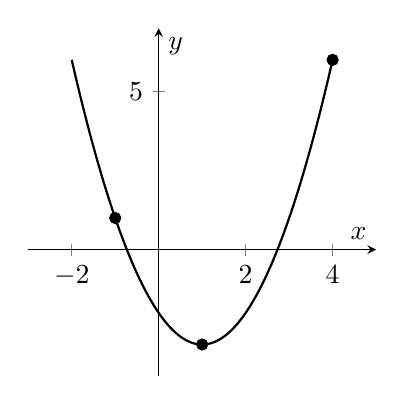
\begin{tikzpicture}
            \begin{axis}[
            xlabel={$x$},
            ylabel={$y$},
            xmin=-3,
            xmax=5,
            ymin=-4,
            ymax=7,
            axis lines=center,
            width=6cm,
            height=6cm]
                \addplot[thick, samples=200, domain=-2:4] {x^2-2*x-2};
                \addplot[
                    color=black,
                    mark=*,
                    only marks
                    ]
                coordinates {
                (-1,1) (1,-3) (4,6)
                };
            \end{axis}
        \end{tikzpicture}
        %\captionof{figure}{Gráfica de la parábola $y=-2-2x+x^2$}
    \end{center}
\end{example}

\newpage

\section{Ejercicios}

\noindent
En los problemas 1 al 16 calcule el determinante.
\begin{tasks}[
    style=enumerate,
    label-offset = 3mm,
    ](2)
    \task $\begin{vmatrix*}[r]7 & 9 & -5 \\ 9 & 3 & 1 \\ -8 & -8 & 10\end{vmatrix*}$
    \task $\begin{vmatrix*}1 & 0 & 3 \\ 0 & 1 & 4 \\ 2 & 1 & 0\end{vmatrix*}$
    \task $\begin{vmatrix*}[r]-1 & 1 & 0 \\ 2 & 1 & 4 \\ 1 & 5 & 6\end{vmatrix*}$
    \task $\begin{vmatrix*}[r]10 & 10 & -8 \\ -7 & 0 & -2 \\ 10 & 6 & 9\end{vmatrix*}$
    \task $\begin{vmatrix*}[r]3 & -1 & 4 \\ 6 & 3 & 5 \\ 2 & -1 & 6\end{vmatrix*}$
    \task $\begin{vmatrix*}[r]-1 & 0 & 6 \\ 0 & 2 & 4 \\ 1 & 2 & -3\end{vmatrix*}$
    \task $\begin{vmatrix*}[r]6 & -10 & 4 \\ 10 & 7 & 5 \\ 3 & 9 & 5\end{vmatrix*}$
    \task $\begin{vmatrix*}[r]-2 & 3 & 1 \\ 4 & 6 & 5 \\ 0 & 2 & 1\end{vmatrix*}$
    \task $\begin{vmatrix*}[r]5 & -2 & 1 \\ 6 & 0 & 3 \\ -2 & 1 & 4\end{vmatrix*}$
    \task $\begin{vmatrix*}[r]-2 & -10 & 7 & 0 \\ 0 & -5 & 4 & -1 \\ 0 & -10 & 0 & 0 \\ 0 & 0 & 0 & 6\end{vmatrix*}$
    \task $\begin{vmatrix*}2 & 0 & 3 & 1 \\ 0 & 1 & 4 & 2 \\ 0 & 0 & 1 & 5 \\ 1 & 2 & 3 & 0\end{vmatrix*}$
    \task $\begin{vmatrix*}[r]-3 & 0 & 0 & 0 \\ -4 & 7 & 0 & 0 \\ 5 & 8 & -1 & 0 \\ 2 & 3 & 0 & 6\end{vmatrix*}$
    \task $\begin{vmatrix*}[r]-6 & 8 & -5 & 0 & 0 \\ 0 & 0 & 0 & 0 & -3 \\ -5 & 0 & -5 & -6 & 0 \\ 0 & -8 & 0 & 0 & 2 \\ 0 & -7 & 0 & 2 & 1\end{vmatrix*}$
    \task $\begin{vmatrix*}[r]2 & 3 & -1 & 4 & 5 \\ 0 & 1 & 7 & 8 & 2 \\ 0 & 0 & 4 & -1 & 5 \\ 0 & 0 & 0 & -2 & 8 \\ 0 & 0 & 0 & 0 & 6\end{vmatrix*}$
    \task $\begin{vmatrix*}[r]0 & 0 & 0 & 0 & 0 \\ 0 & 7 & 0 & 0 & 0 \\ -9 & 1 & 0 & 0 & 0 \\ -6 & 0 & 0 & -2 & -7 \\ 9 & -9 & 0 & -5 & 0\end{vmatrix*}$
    \task $\begin{vmatrix*}[r]-8 & 0 & 0 & -10 & 0 \\ 0 & -8 & 0 & -7 & 1 \\ 0 & 9 & -3 & 0 & -4 \\ -5 & 0 & 7 & 5 & 5 \\ -2 & 0 & -10 & 3 & -7\end{vmatrix*}$
\end{tasks}
\begin{enumerate}[start=17]
    \item Si existe, calcule la matriz inversa de las anteriores matrices mediante la expresión \ref{ADJUNTODEMATRIZ}.
    \item Demuestre que si $A$ y $B$ son matrices diagonales de $n \times n$, entonces $\Det A B=\Det A \Det B$.
    \item Demuestre que si $A$ y $B$ son matrices triangulares inferiores, entonces $A B=\Det A \Det B$.
    \item Demuestre que, en general, no se cumple que $\Det(A+B)=\Det A+\Det B$.
    \item Muestre que si $A$ es triangular, entonces $\Det A \neq 0$ si y sólo si todos los elementos en la diagonal de $A$ son diferentes de cero.
\end{enumerate}
De los problemas 22 al 30 calcule el determinante suponiendo que
$$
\begin{vmatrix*}
a_{11} & a_{12} & a_{13} \\
a_{21} & a_{22} & a_{23} \\
a_{31} & a_{32} & a_{33}
\end{vmatrix*}=8
$$\newpage
\begin{tasks}[
    start=22,
    style=enumerate,
    label-offset = 3mm,
    ](2)
    \task $\begin{vmatrix*}a_{31} & a_{32} & a_{33} \\ a_{21} & a_{22} & a_{23} \\ a_{11} & a_{12} & a_{13}\end{vmatrix*}$
    \task $\begin{vmatrix*}a_{31} & a_{32} & a_{33} \\ a_{11} & a_{12} & a_{13} \\ a_{21} & a_{22} & a_{23}\end{vmatrix*}$
    \task $\begin{vmatrix*}a_{11} & a_{13} & a_{12} \\ a_{21} & a_{23} & a_{22} \\ a_{31} & a_{33} & a_{32}\end{vmatrix*}$
    \task $\begin{vmatrix*}a_{11} & a_{12} & a_{13} \\ 2 a_{21} & 2 a_{22} & 2 a_{23} \\ a_{31} & a_{32} & a_{33}\end{vmatrix*}$
    \task $\begin{vmatrix*}[r]-3 a_{11} & -3 a_{12} & -3 a_{13} \\ 2 a_{21} & 2 a_{22} & 2 a_{23} \\ 5 a_{31} & 5 a_{32} & 5 a_{33}\end{vmatrix*}$
    \task $\begin{vmatrix*}4 a_{11} & -2 a & 3 a_{12} \\ 4 a_{21} & -2 a_{23} & 3 a_{22} \\ 4 a_{31} & -2 a_{33} & 3 a_{32}\end{vmatrix*}$
    \task $\begin{vmatrix*}a_{11} & 2 a_{13} & a_{12} \\ a_{21} & 2 a_{23} & a_{22} \\ a_{31} & 2 a_{33} & a_{32}\end{vmatrix*}$
    \task $\begin{vmatrix*}a_{11} & -a_{12} & a_{12} & a_{13} \\ a_{21} & -a_{22} & a_{22} & a_{23} \\ a_{31} & -a_{32} & a_{32} & a_{33}\end{vmatrix*}$
    \task $\begin{vmatrix*}2 a_{11}-3 a_{21} & 2 a_{12}-3 a_{22} & 2 a_{13}-3 a_{23} \\ a_{31} & a_{32} & a_{33} \\ a_{21} & a_{22} & a_{23}\end{vmatrix*}$
\end{tasks}
\begin{enumerate}[start=31]
    \item Demuestre que si $\alpha$ es un escalar y $A$ es una matriz cuadrada de tamaño $n \times n$, entonces $\Det(\alpha A)=\alpha^n \Det(A)$.
    \item Demuestre que
    $$\begin{vmatrix}
        1+x_1 & x_2 & x_3 & \cdots & x_n \\
        x_1 & 1+x_2 & x_3 & \cdots & x_n \\
        x_1 & x_2 & 1+x_3 & \cdots & x_n \\
        \vdots & \vdots & \vdots & & \vdots \\
        x_1 & x_2 & x_3 & \cdots & 1+x_n
    \end{vmatrix} = 1+x_1+x_2+\cdots+x_n$$
    \item Demuestre que
    $$\begin{vmatrix*}
        \lambda & -1 & 0 & \cdots & 0 & 0 & 0 \\
        0 & \lambda & -1 & \cdots & 0 & 0 & 0 \\
        0 & 0 & \lambda & \ddots & 0 & 0 & 0 \\
        \vdots & \vdots & \vdots & \ddots & \vdots & \vdots & \vdots \\
        0 & 0 & 0 & \cdots & \lambda & -1 & 0 \\
        0 & 0 & 0 & \cdots & 0 & \lambda & -1 \\
        a_0 & a_1 & a_2 & \cdots & a_{n-3} & a_{n-2} & \lambda+a_{n-1}
    \end{vmatrix*}=\lambda^n+a_{n-1} \lambda^{n-1}+a_{n-2} \lambda^{n-2}+\cdots+a_1 \lambda^1+a_0$$
    \item Sea $A$ una matriz de $n \times n$. Demuestre que si la suma de todos los elementos de cada columna de $A$ es cero, entonces $|A|=0$.
    \item Una matriz $A$ es antisimétrica si $A^{T}=-A$ (definición \ref{matriz-antisimetrica}). Si $A$ es una matriz antisimétrica de $n \times n$, demuestre que $\Det A^{T}=(-1)^n \Det A$.
    \item Usando el resultado del problema anterior, demuestre que si $A$ es una matriz antisimétrica de $n \times n$ y $n$ es impar, entonces $\Det A=0$.
    \item Una matriz $A$ se llama ortogonal si $A$ es invertible y $A^{-1}=A^{T}$, es decir, $A^{T} A=A A^{T}=I$. Demuestre que si $A$ es ortogonal, entonces $\Det A= \pm 1$.
    \item La matriz $A$ se llama idempotente si $A^2 = A$ (definición \ref{def:matriz-idempotente}). ¿Cuáles son los valores posibles para $\Det A$ si $A$ es idempotente?
    \item Si es posible, resuelva los sistemas de la página \pageref{EJERCICIOSDECRAMER} usando la regla de Cramer.
\end{enumerate}